% !TeX root = ../../ZF_bmicha_Ana.tex
\subsection{Flächenberechnungen}
    \vspace{0.5em}
    \begin{itemize}
        \item Parametrisierung $\vec{r}=(x(t),y(t))^T$ \hfill
    \end{itemize}
    \begin{minipage}{0.65\linewidth}
        \vspace{-1em}
        \begin{itemize}
        \item[]  $\displaystyle A= \underbrace{\int_{t_1}^{t_2} + y \dot{x} \, dt}_{x \textrm{ monoton steigend}}$
        \item[]  $\displaystyle A= \underbrace{\int_{t_1}^{t_2} - y \dot{x} \, dt}_{x \textrm{ monoton fallend}}$
        \end{itemize}
    \end{minipage}
    \begin{minipage}{0.34\linewidth}
        
\includegraphics[width=0.7\linewidth]{src/11_Integralrechnung/param.pdf}
    \end{minipage}

    \subsubsection{Sektorfläche}
        \flushleft Fläche zwischen Ursprung und Kurve
        \begin{minipage}{0.99\linewidth}
            \begin{minipage}{0.65\linewidth}
                \begin{itemize}
                    \item Parametrisierung
                    \item[]  $\displaystyle A= \frac{1}{2} \int_{t_1}^{t_2} (x \dot{y} - y \dot{x}) \, dt$   
                    \end{itemize}
            \end{minipage}
            \begin{minipage}{0.34\linewidth}
                    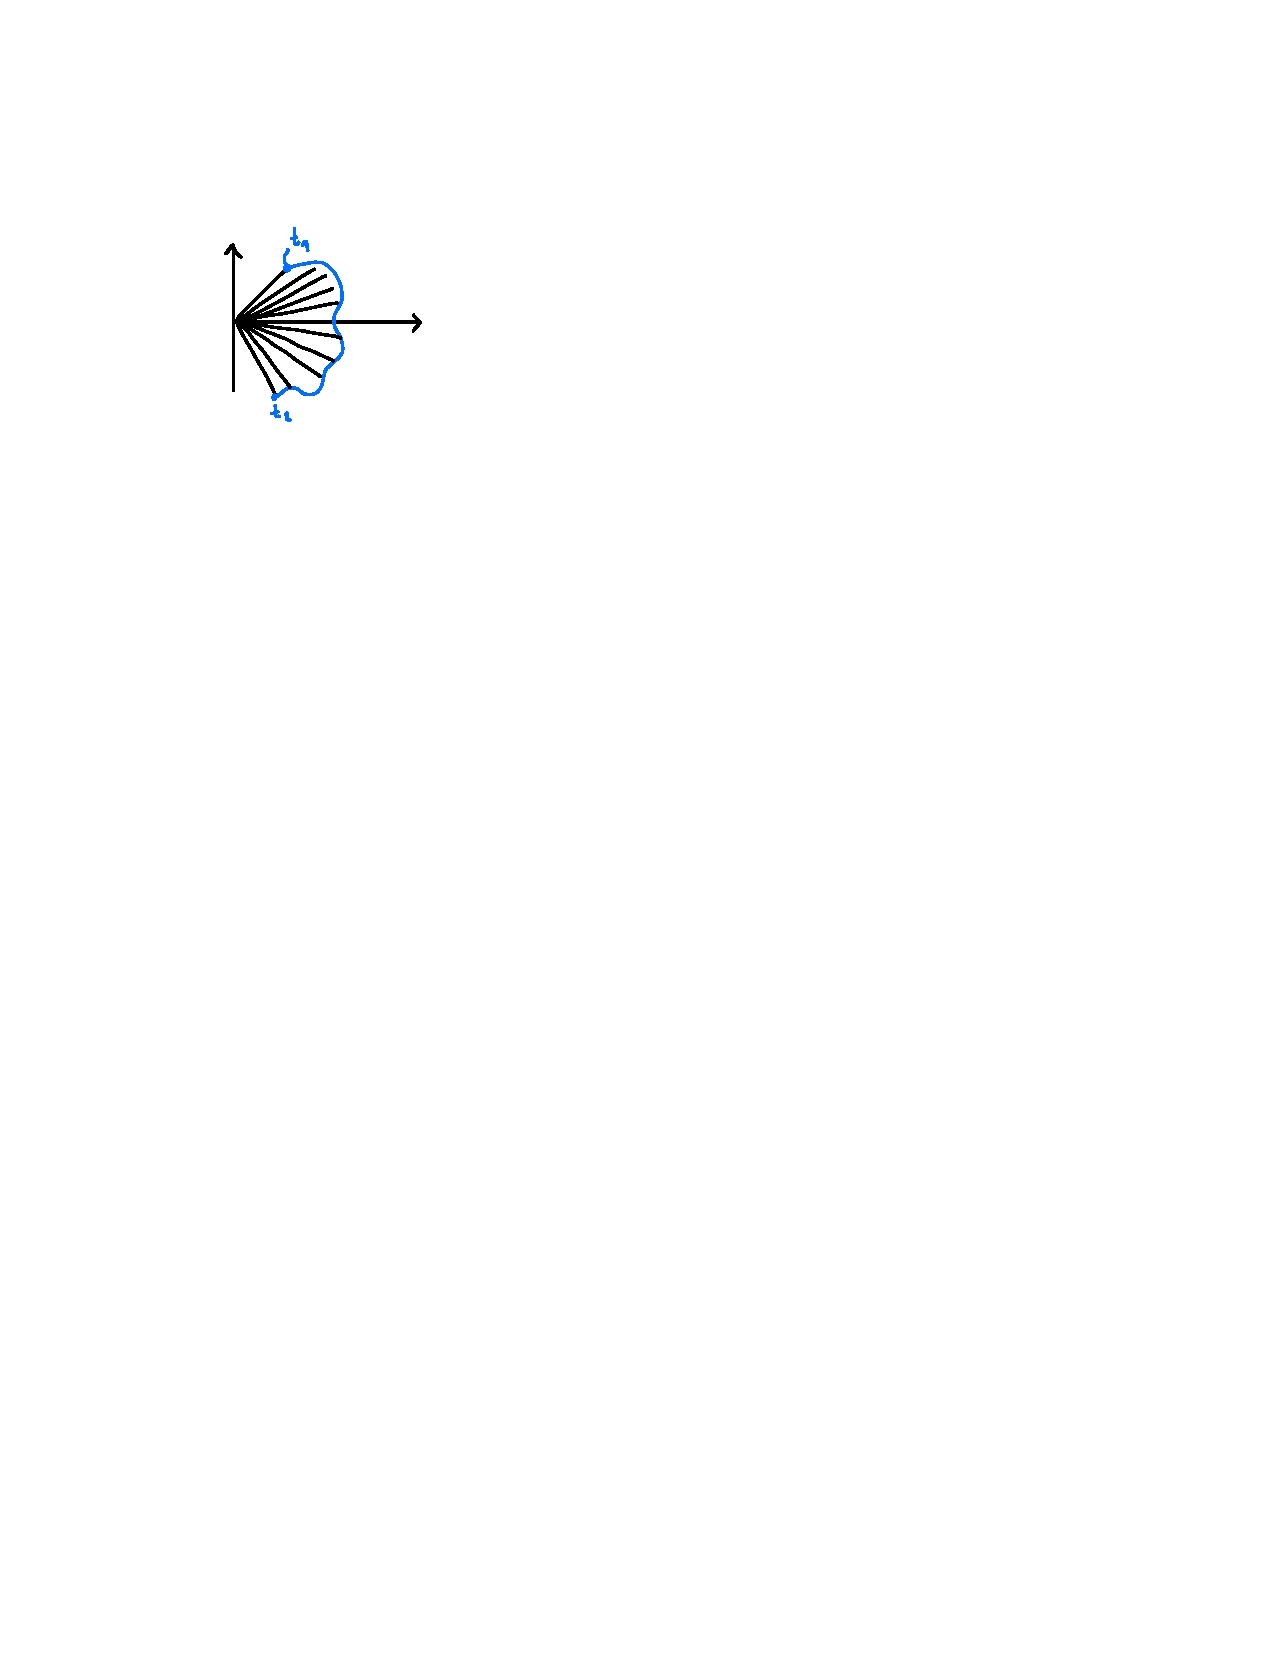
\includegraphics[width=0.6\linewidth]{src/11_Integralrechnung/sektor.pdf}
            \end{minipage}
        \end{minipage}
        
        \begin{minipage}{0.99\linewidth}
            \begin{minipage}{0.65\linewidth}
                \begin{itemize}
                    \item Polarkoordinaten
                    \item[] $ \displaystyle A= \frac{1}{2} \int_{\varphi_1}^{\varphi_2} \rho^2(\varphi) \, d\varphi $
                \end{itemize}
            \end{minipage}
            \begin{minipage}{0.34\linewidth}
                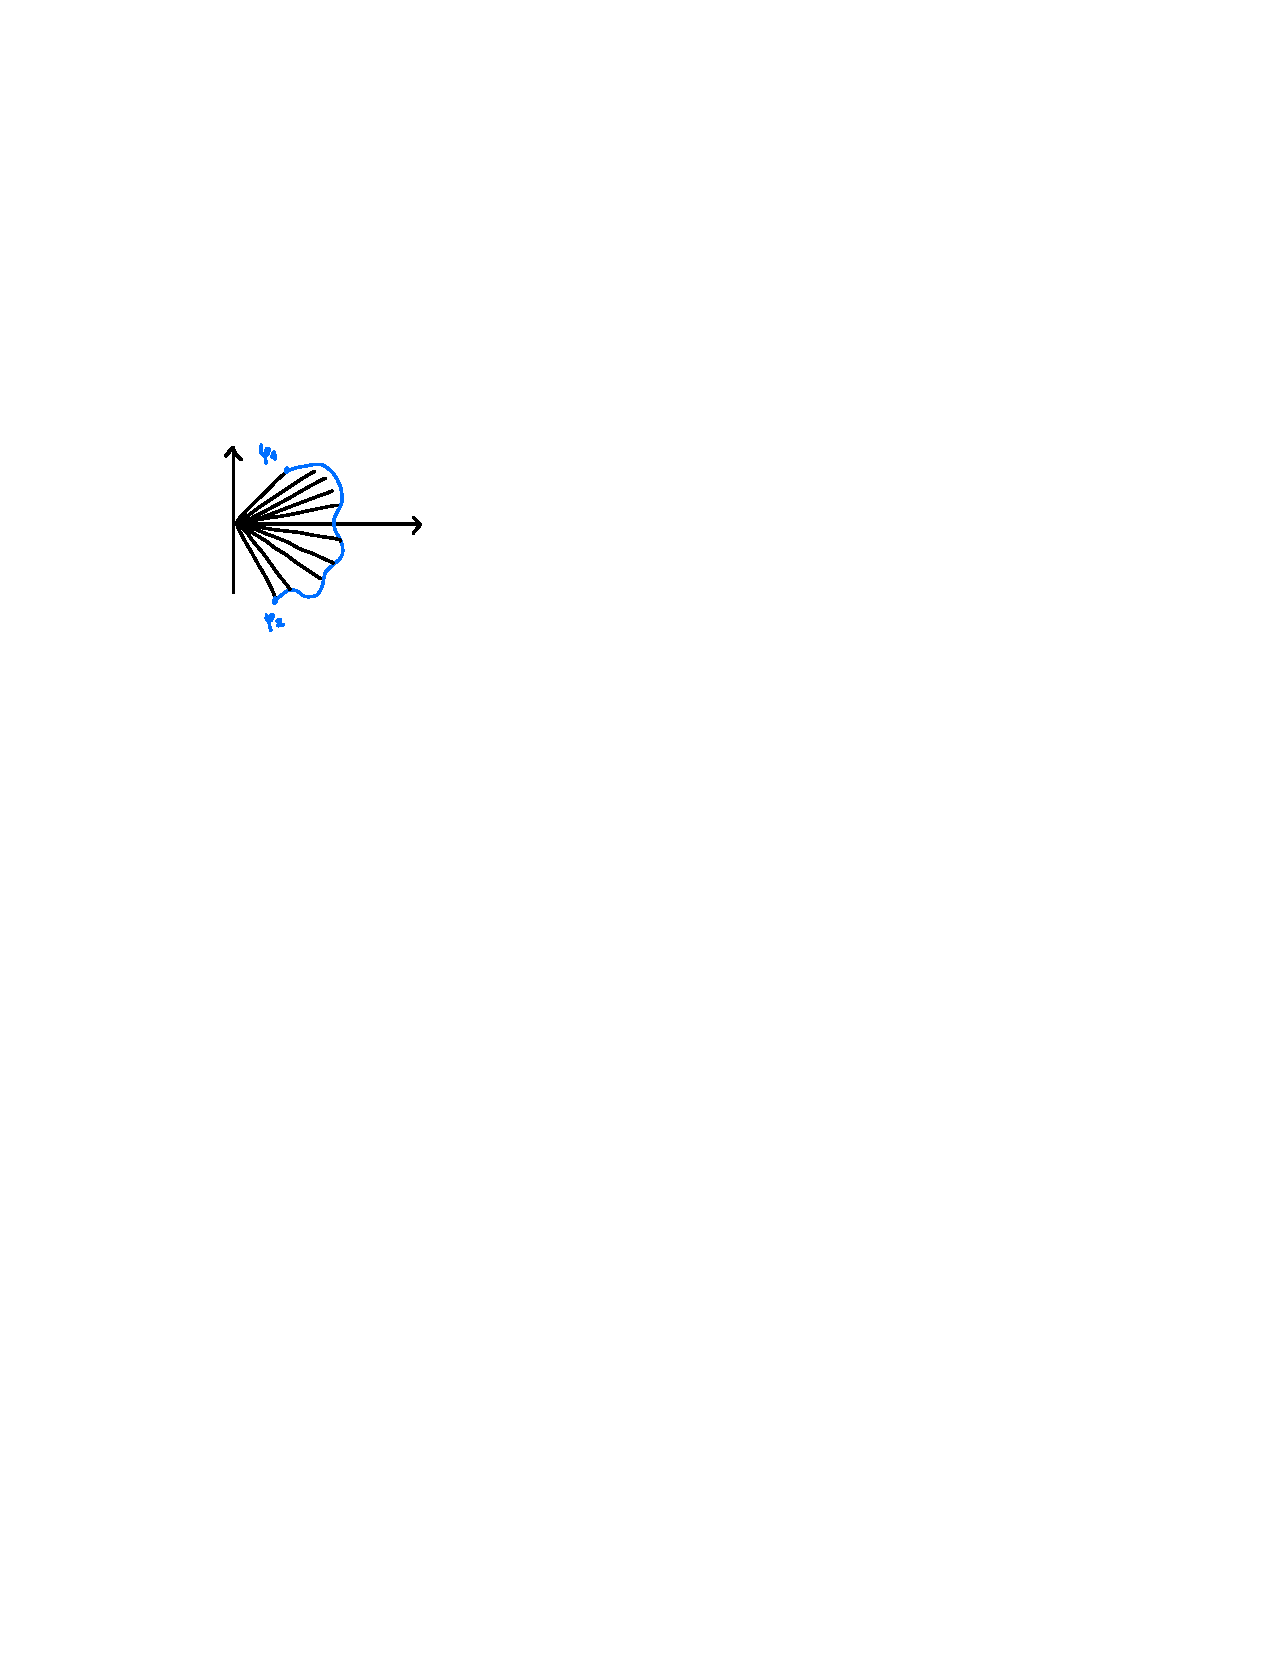
\includegraphics[width=0.6\linewidth]{src/11_Integralrechnung/polar.pdf}
            \end{minipage}
        \end{minipage}
        {\scriptsize Fläche auf der rechten Seite der Kurve hat positives Vorzeichen.}